\documentclass[10pt,letterpaper]{article} 
\usepackage{tikz}
\usepackage{tools}
\usepackage{enumitem,caption}
\usepackage{listings}
\lstset{language=Python}
%\lstset{frame=lines}
%\lstset{caption={Insert code directly in your document}}
\lstset{label={lst:code_direct}}
\lstset{basicstyle=\footnotesize}

%\usepackage{graphicx}‎‎
%\usefonttheme{serif}‎
%\usepackage{ptext}‎
%\usepackage{xepersian}
%\settextfont{B Nazanin}
\usepackage{lipsum}
\setlength{\parindent}{0pt}
\newcommand{\pf}{$\blacksquare$}

\newcommand{\Span}{\text{Span}}
\newcommand{\NF}{\text{NF}}
\newcommand{\EDFA}{\text{EDFA}}
\newcommand{\ASE}{\text{ASE}}

\newcommand{\bns}{\textit{broadcast-and-select}  architecture}
\newcommand{\Bns}{\textit{Broadcast-and-select} architecture}

\newcommand{\rns}{\textit{route-and-select} architecture}
\newcommand{\Rns}{\textit{Route-and-select} architecture}

\newcounter{QuestionNumber}
\setcounter{QuestionNumber}{1}

\newcommand{\temp}{{\color{red}{temp}}}

\newcommand{\Q}{
\textbf{Question \theQuestionNumber)}
\stepcounter{QuestionNumber}
}
\newcommand{\EX}{\Bbb E}
\newcommand{\nl}{\newline\newline}
\begin{document}
\large
\begin{center}
In the name of beauty

The 5th problem set of Optical Networks course
\hl
\end{center}
\Q
(Linear Programming)

Solve the following linear programmings by sketching the feasible region.
\begin{enumerate}[label=\alph*-]
\item
\qn{
&\text{maximize}\ \  3x_1+2x_2
\\& \text{subject to}
\\& \ \ \ \ \ \ x_1+2x_2\le 7
\\& \ \ \ \ \ \ x_1-x_2\le 1
\\& \ \ \ \ \ \ x_1+x_2\ge 1
\\& \ \ \ \ \ \ x_2\le 3
\\& \ \ \ \ \ \ 0\le x_1\le 2
}
\item
\qn{
&\text{minimize}\ \  5x_1+x_2
\\& \text{subject to}
\\& \ \ \ \ \ \ 5x_1+x_2\ge 2
\\& \ \ \ \ \ \ x_2\ge {x_1}/{2}
\\& \ \ \ \ \ \ 7x_1+5x_2\le 19
\\& \ \ \ \ \ \ x_2\le 2-6x_1
%\\& \ \ \ \ \ \ 0\le x_1\le 2
}
\item
\qn{
&\text{minimize}\ \  4x_1-3x_2
\\& \text{subject to}
\\& \ \ \ \ \ \ x_2\le x_1+1
\\& \ \ \ \ \ \ 2x_1+3x_2\le 13
\\& \ \ \ \ \ \ 5x_2\ge 11x_1-50
%\\& \ \ \ \ \ \ 0\le x_1\le 2
}
\end{enumerate}

\Q
(Integer Linear Programming)

Solve the following integer linear programmings by sketching the feasible region.
\begin{enumerate}[label=\alph*-]
\item
\qn{
&\text{maximize}\ \  x_1+x_2
\\& \text{subject to}
\\& \ \ \ \ \ \ x_2\le 2x_1+3
\\& \ \ \ \ \ \ 2x_1-4x_2+15\ge 0
\\& \ \ \ \ \ \ x_2+10x_1-42\le 1
\\& \ \ \ \ \ \ x_1,x_2\in\mathbb{Z}
}
\item
\qn{
&\text{maximize}\ \  7x_1+4x_2
\\& \text{subject to}
\\& \ \ \ \ \ \ 7x_1+4x_2\le 35
\\& \ \ \ \ \ \ 2x_2\le x_1+4
\\& \ \ \ \ \ \ x_2\ge0
\\& \ \ \ \ \ \ x_1,x_2\in\mathbb{Z}
}
\end{enumerate}

\Q

\begin{enumerate}[label=\alph*-]
\item
What problem could emerge in Bellman-Ford algorithm for finding shortest path between two nodes if there is a negative loop in a network (a negative loop is a sequence of links with negative costs over which traffic could travel)?
\item
Apply Dijkstra's algorithm on the two following networks to find the minimum-cost path between nodes A and B.
\item
Apply Bellman-Ford's algorithm to network of figure (\ref{bf}) to find the shortest path between nodes A and B. Why is your answer different from that of part -a-?
\end{enumerate}
\begin{figure}[h]
\centering
\begin{subfigure}{0.48\textwidth}
\centering
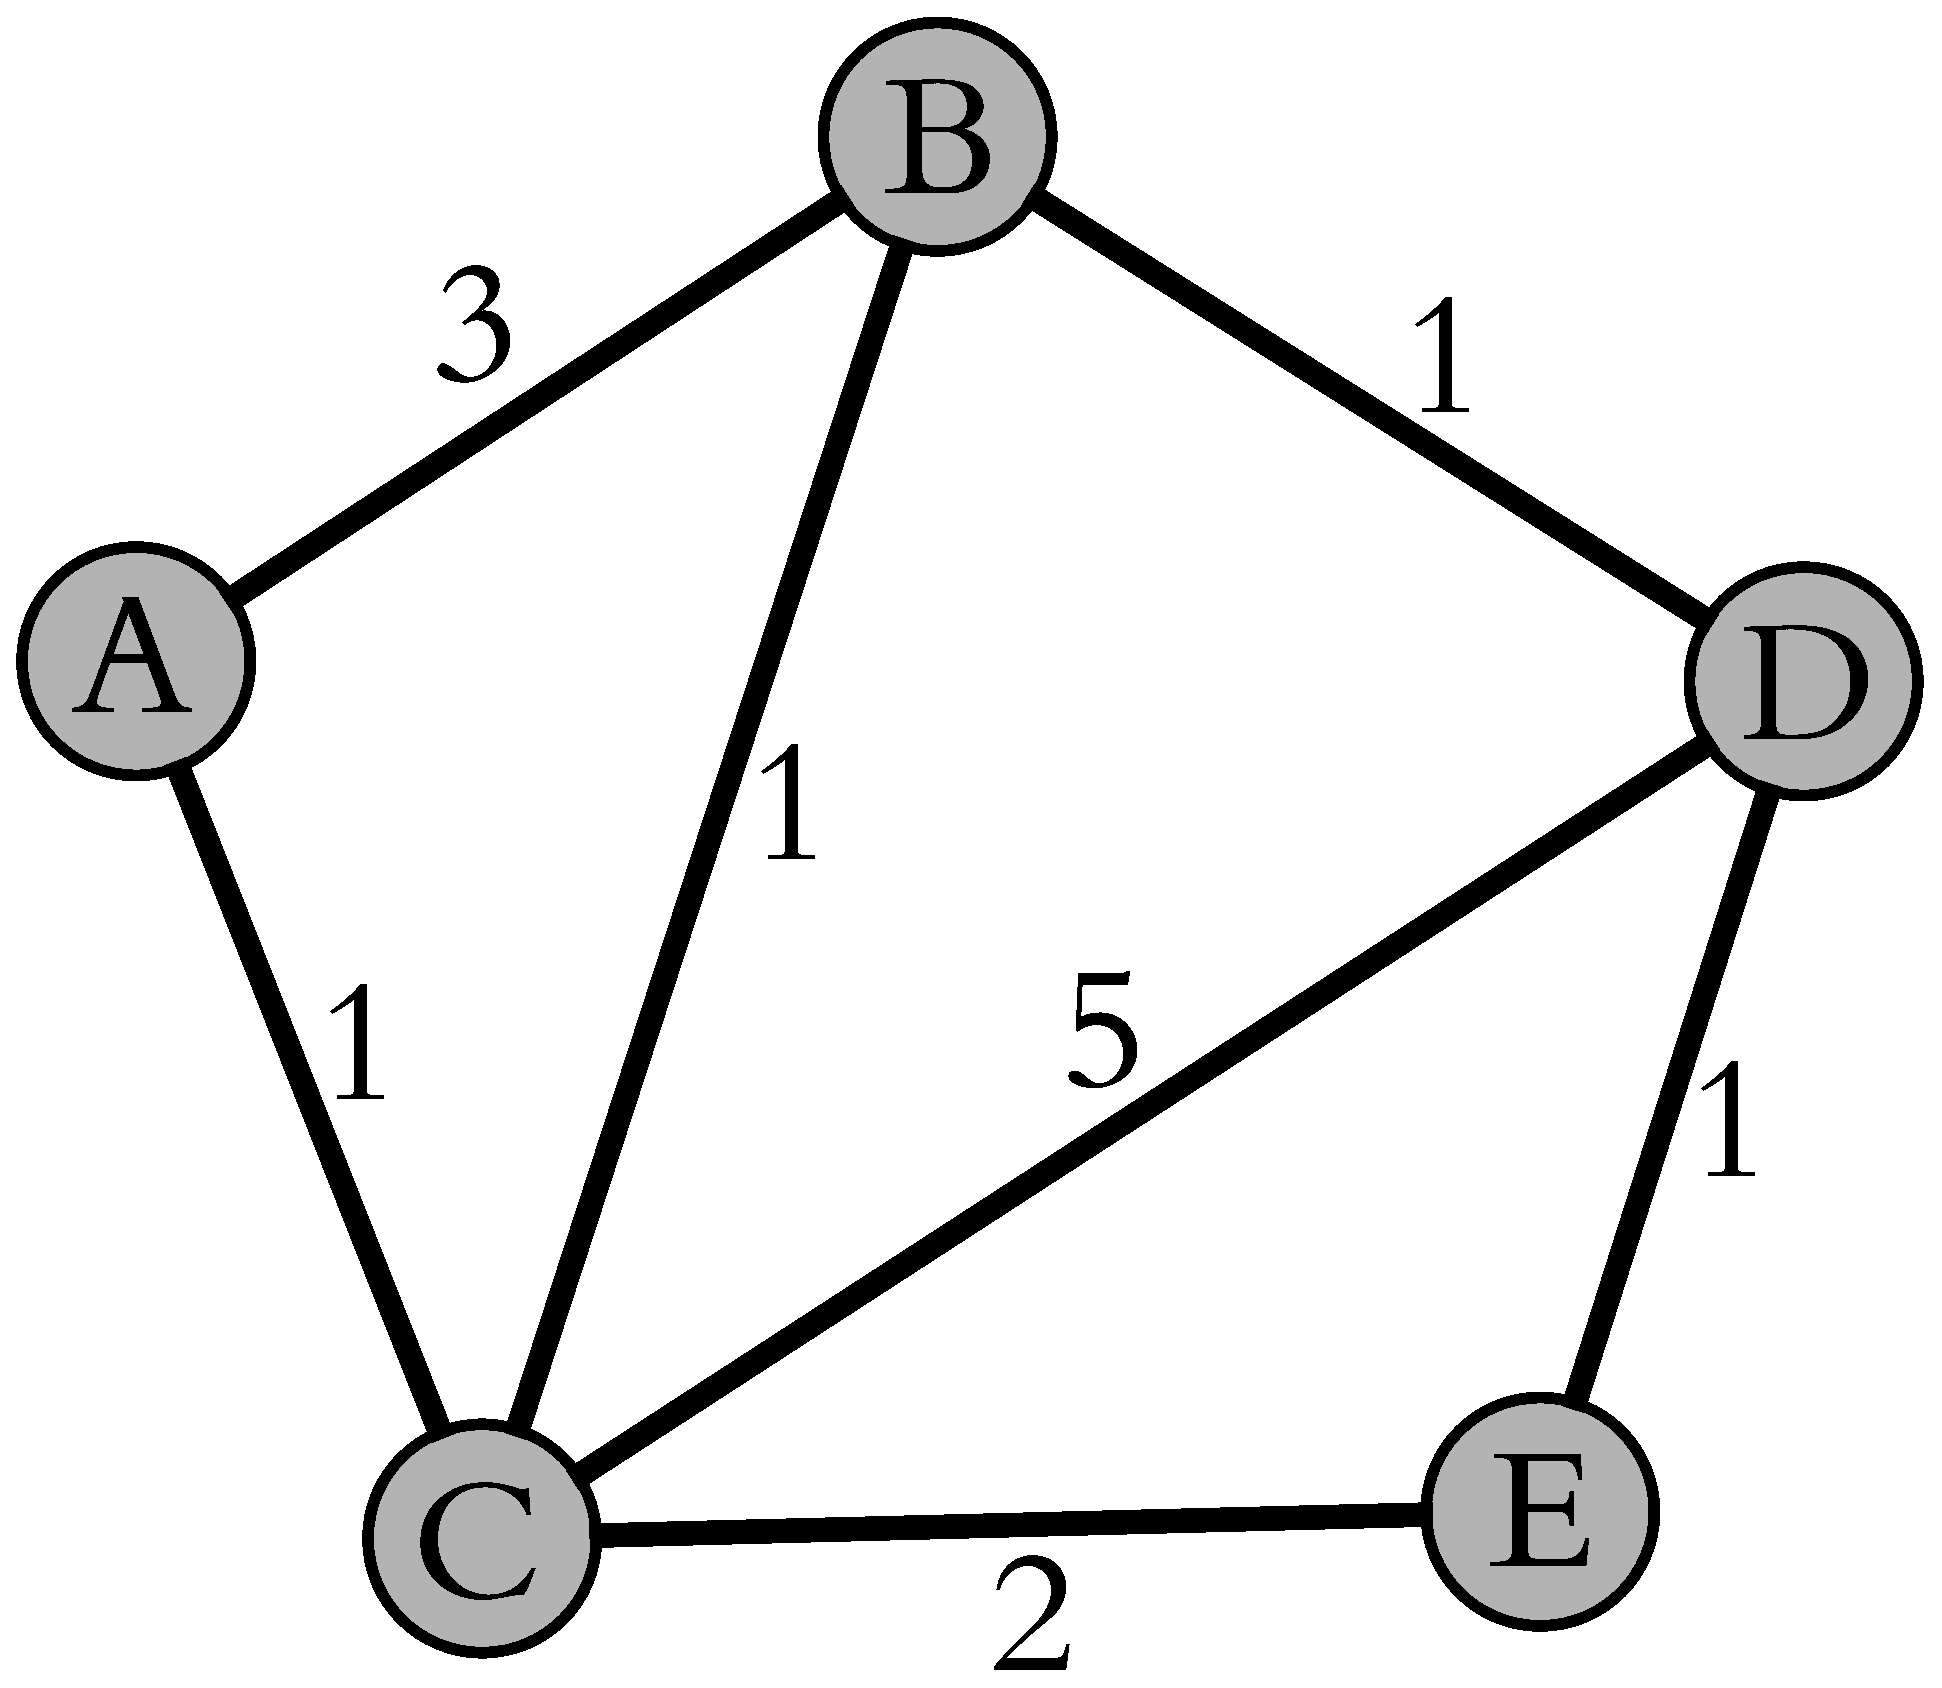
\includegraphics[width=50mm]{Dijkstra.eps}
\caption{Simple network}
\end{subfigure}
\begin{subfigure}{0.48\textwidth}
\centering
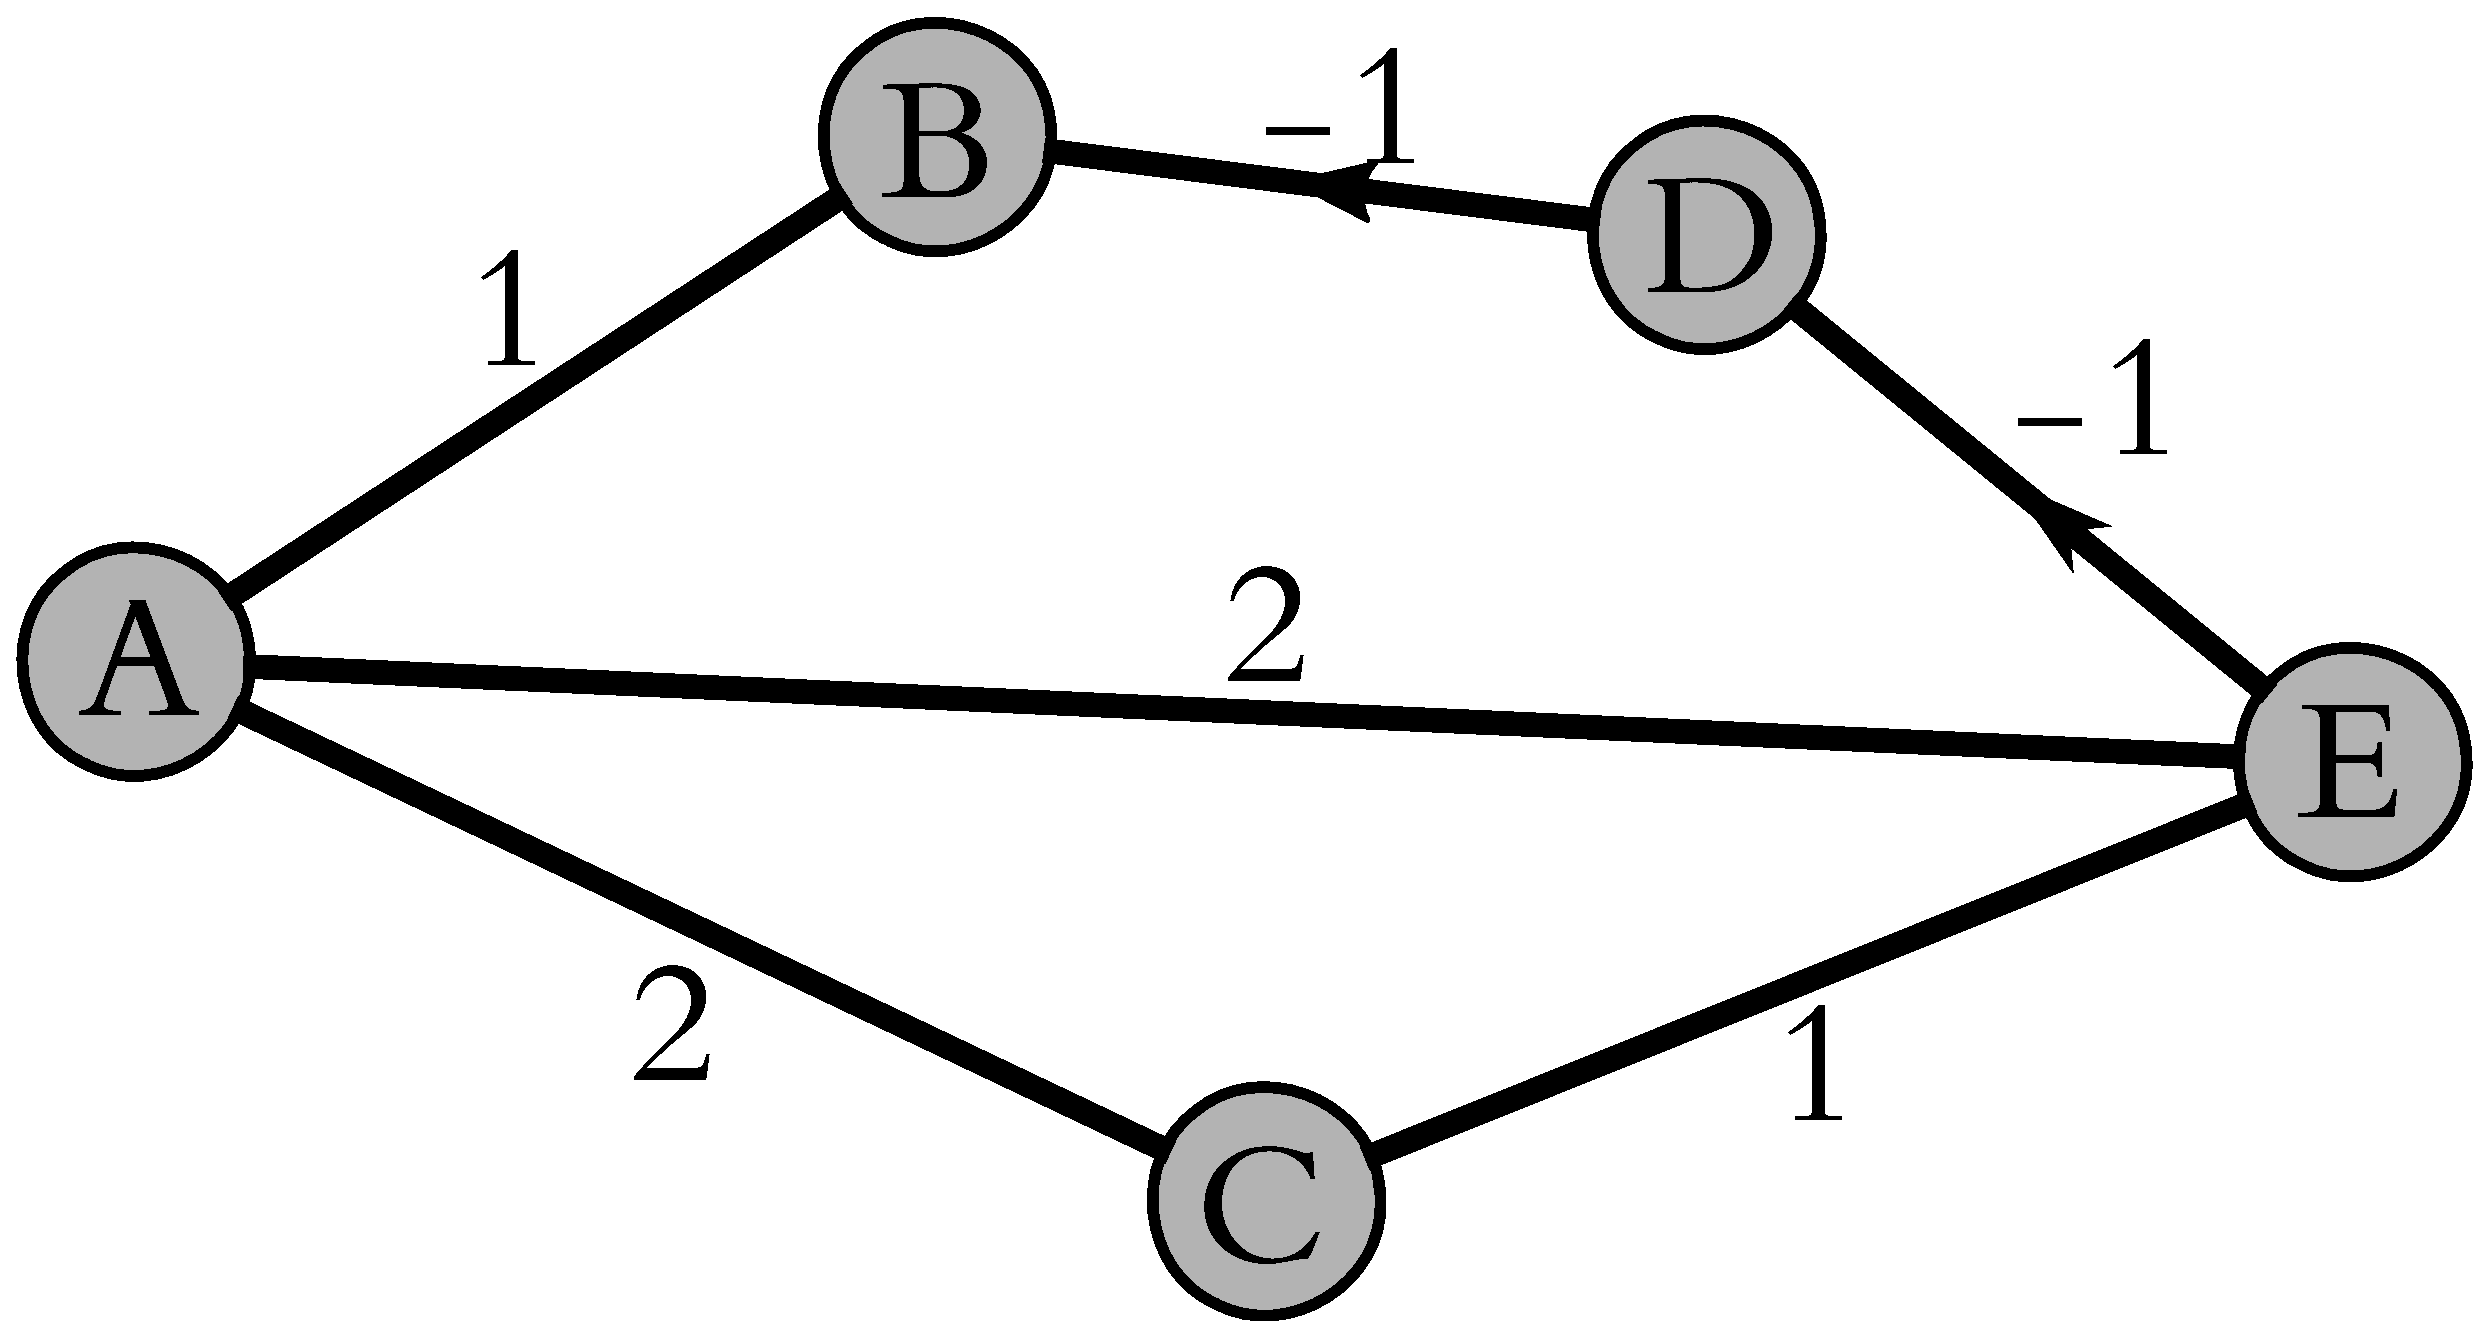
\includegraphics[width=65mm]{Dijkstra_Flawed.eps}
\caption{Network with positive and negative link costs}
\label{bf}
\end{subfigure}
\caption{}
\end{figure}

\Q

We wish to solve the max-flow problem in the following network through LP. Our objective is the maximal flow that can traverse the following physical topology.
\begin{figure}[h]
\centering
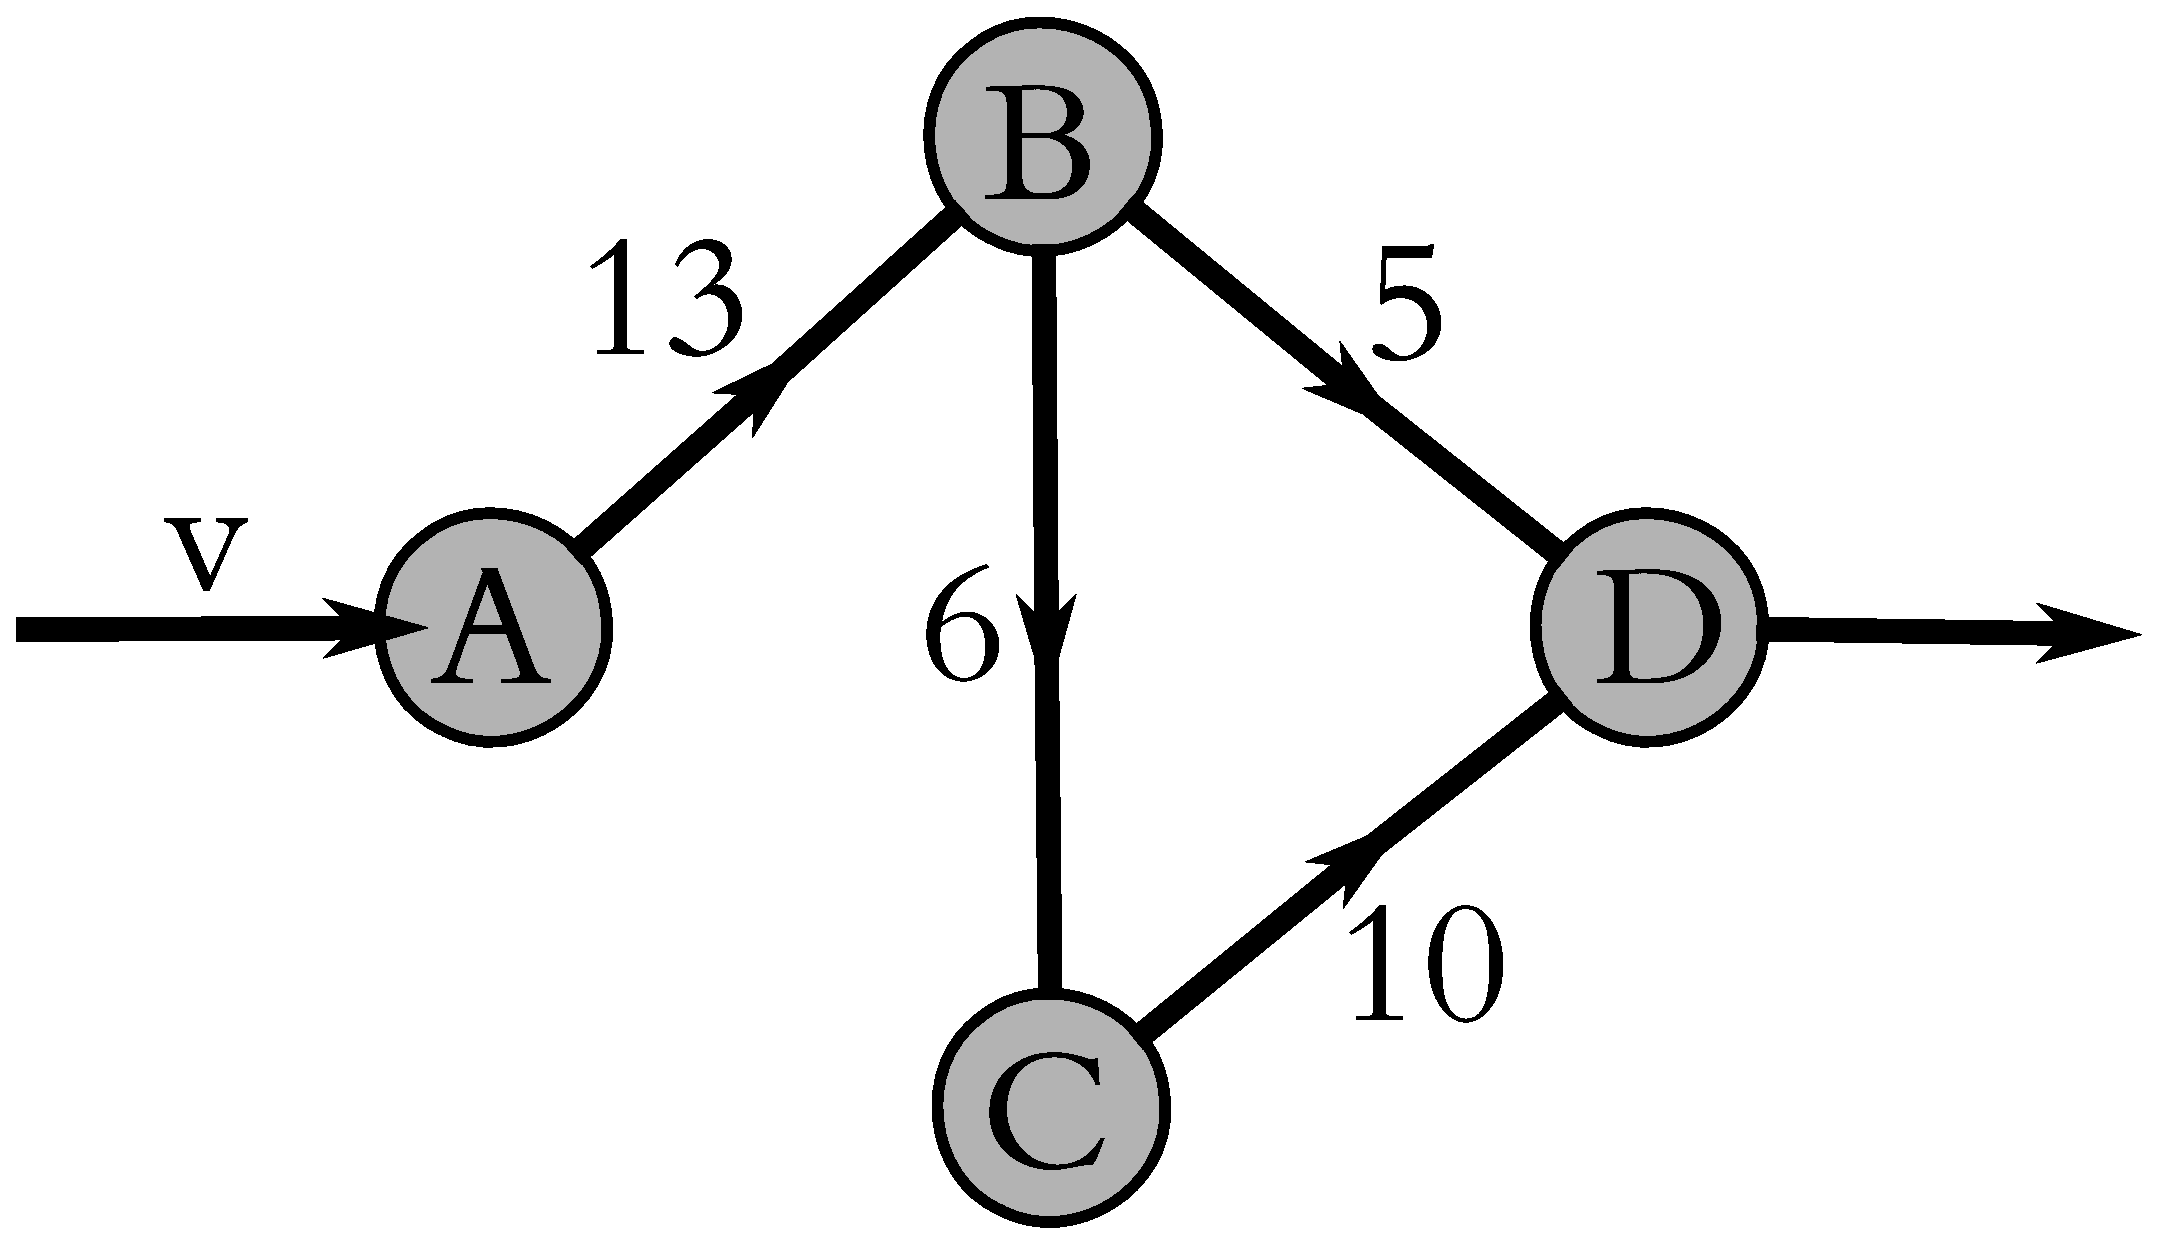
\includegraphics[width=60mm]{max_flow.eps}
\end{figure}
The numbers on each link denote the capacity of the link. Assume the total flow from node i to node j on their direct link is $x_\text{ij}$ and each such flow must not exceed its capacity and is always non-negative, e.g.
$
0\le x_\text{BC} \le 6.
$
The total traffic volume $v$ passes through this network from node A to node D, which should be maximized. Formulate the problem of maximum flow in LP framework and solve it to find the maximum traffic. Section 4.2.1 of ``Linear Programming and Algorithms for Communication Networks'' has discussed this type of LP problems in detail (further simplifications on the problem formulation would leave you with a two-dimensional LP, so you can solve it visually).


\end{document}